%%%%%%%%%%%%%%%%%%%%%%%%%%%%%%%%%%%%%%%%%%%%%%%%%%%%%%%%%%%%%%%%%%%%%%%%%%%%%%%%
% IEEE RA-L INITIAL-SUBMISSION WORKING PAPER
% Double-anonymous draft: do not add authors, affiliations, acknowledgments,
% repository URLs, or other identifying metadata before review submission.
%%%%%%%%%%%%%%%%%%%%%%%%%%%%%%%%%%%%%%%%%%%%%%%%%%%%%%%%%%%%%%%%%%%%%%%%%%%%%%%%

\documentclass[letterpaper,10 pt,conference]{ieeeconf}

\IEEEoverridecommandlockouts
\overrideIEEEmargins

\usepackage{amsmath}
\usepackage{amssymb}
\usepackage{bm}
\usepackage{booktabs}
\usepackage{cite}
\usepackage{graphicx}
\usepackage{url}

\newcommand{\R}{\mathbb{R}}
\newcommand{\ind}{\mathbf{1}}
\newcommand{\clip}{\operatorname{clip}}
\newcommand{\softmax}{\operatorname{softmax}}
\newcommand{\dS}{d_{S^1}}
\newcommand{\pgso}{\textsc{PGS-O}}
\newcommand{\pgsg}{\textsc{PGS-G}}
% Keep the audited 34-entry bibliography within the conference page budget.
\newcommand{\BIBdecl}{\scriptsize}
\newtheorem{proposition}{Proposition}

\title{\LARGE \bf
Learning-Based Tactile Posterior-Guided Search for Robotic Hex-Socket Engagement
}

% RA-L initial submissions are double anonymous.  The empty box intentionally
% leaves the author byline blank while retaining the template's title spacing.
\author{\mbox{}}

\begin{document}

\maketitle
\thispagestyle{empty}
\pagestyle{empty}

%%%%%%%%%%%%%%%%%%%%%%%%%%%%%%%%%%%%%%%%%%%%%%%%%%%%%%%%%%%%%%%%%%%%%%%%%%%%%%%%
\begin{abstract}
Hex-socket unscrewing starts with one small move: the driver must enter the
socket before torque can be applied.  Visual alignment brings the tool close
to the screw head, but the residual error can still match the chamfer
capture range.  An outward spiral search is safe against this error, but it
keeps checking locations that contact has already ruled out.  A single
learned move covers less ground, but it is unsafe when touch shows direction
better than it shows distance.  This paper builds a search that uses both
ideas together.  A low-force conical probe records axial force, bending
torque, and tip height while it moves.  A trained ensemble turns this signal
into a direction estimate and a contact-confidence estimate.  These two
estimates reweight a CAD prior over the socket center.  The confident part
of that estimate becomes a short, capped move, and the rest goes to a small
local search.  Capture, recovery, force limits, and the final check all run
through one compliant control loop.  In paired M8 simulations, this method
keeps the same engagement rate as outward search, with a shorter path and
less time.  Tests on M10 and M12 sockets, and trials on a KUKA LBR iiwa,
show the same method still works at other sizes.  Learned touch, in short,
is useful here mainly for choosing where to search, not for deciding that
the driver has already engaged.
\end{abstract}

\noindent\textbf{Index Terms---}Learning-based control, tactile sensing,
robotic unscrewing, active perception, contact-rich manipulation, compliant
interaction.

%%%%%%%%%%%%%%%%%%%%%%%%%%%%%%%%%%%%%%%%%%%%%%%%%%%%%%%%%%%%%%%%%%%%%%%%%%%%%%%%
\section{Introduction}

Hex-socket unscrewing is usually treated as a torque-control problem.  But
many trials are actually decided before the screw is even turned.  The
driver first has to enter a recessed socket, and the clearance there is
small compared with the residual error of a camera--CAD
estimate~\cite{diaz2025unscrewing}.  Going down too early lands on the screw
head.  Searching from scratch is safer, but it wastes contact travel on
locations that the first touch has already ruled out.  This is a familiar
part-mating problem~\cite{whitney1982quasistatic,lian2021benchmarking}.
Here it comes with one more constraint: the search must finish inside a
short manipulation cycle.

Compliance is the usual first defense against this kind of error.
Remote-center compliance and impedance control let the mating geometry fix
small misalignments on its
own~\cite{whitney1982quasistatic,hogan1985impedance}.  When the offset is
larger, though, the controller also has to decide where to touch next.
Belief-space planning has been used for
this~\cite{wirnshofer2020partial,chintalapudi2026bilevel,noseworthy2025forge}.
Contact-implicit and complementarity methods instead treat the contact mode
as part of the control
problem~\cite{lecleach2024fast,aydinoglu2024consensus,yang2024sliding}.
Fast approximations of contact dynamics give another path to tractable
planning~\cite{carpentier2024contact,graesdal2024convex,suh2026trust}.  Over
the last few millimeters above a socket, though, the question is simpler:
what motion is actually justified by the contact just felt?

Touch alone can answer part of this question, even without a camera on the
contact~\cite{li2020review}.  Contact-pose estimation and active extrinsic
sensing pull compact state estimates out of a prescribed
motion~\cite{jin2021contact,kim2022active}.  Learned tactile and
visuotactile methods push this further, to richer sensors and less
structured
interactions~\cite{calandra2017feeling,lee2019visiontouch,higuera2025sparsh,
zhao2025t3,liang2022tactile,ai2024robopack,oller2024tactile,
ferrandis2025visuotactile,huang2025vitac,yu2025mimictouch,
lin2024touching}.  These works show that touch carries real geometric
information.  None of them, though, says how far a robot should actually
move when that information is still incomplete.

This gap matters for the conical probe used here.  Its wrench pattern
usually points at the bearing of the socket center.  But it is much less
sure about the radial offset.  Treat the bearing as a point estimate, and
the driver can overshoot a small socket.  Ignore it, and the only useful
touch made so far is wasted.  Meta-learned and offline insertion policies
address related adaptation
problems~\cite{schoettler2020meta,zhao2022offline}, and diffusion policies
give strong general visuomotor priors~\cite{chi2023diffusion}.  Final
engagement still needs explicit force and timing
rules~\cite{chen2025funnel,xue2025predictive,xu2025sequensync}.
Differently, in this work, learning only picks where to search.  It never
gets to decide that the driver has engaged.

Figure~\ref{fig:hardware_frames} shows the setup and the coordinate
convention used below.  The interaction frame sits on the force-sensing
tool.  The fixture frame marks the flat socket geometry.  The robot-base
frame gives the commanded Cartesian reference.  All $z$ axes point up, so
engagement depth grows along $-z_p$.

\begin{figure*}[t]
  \centering
  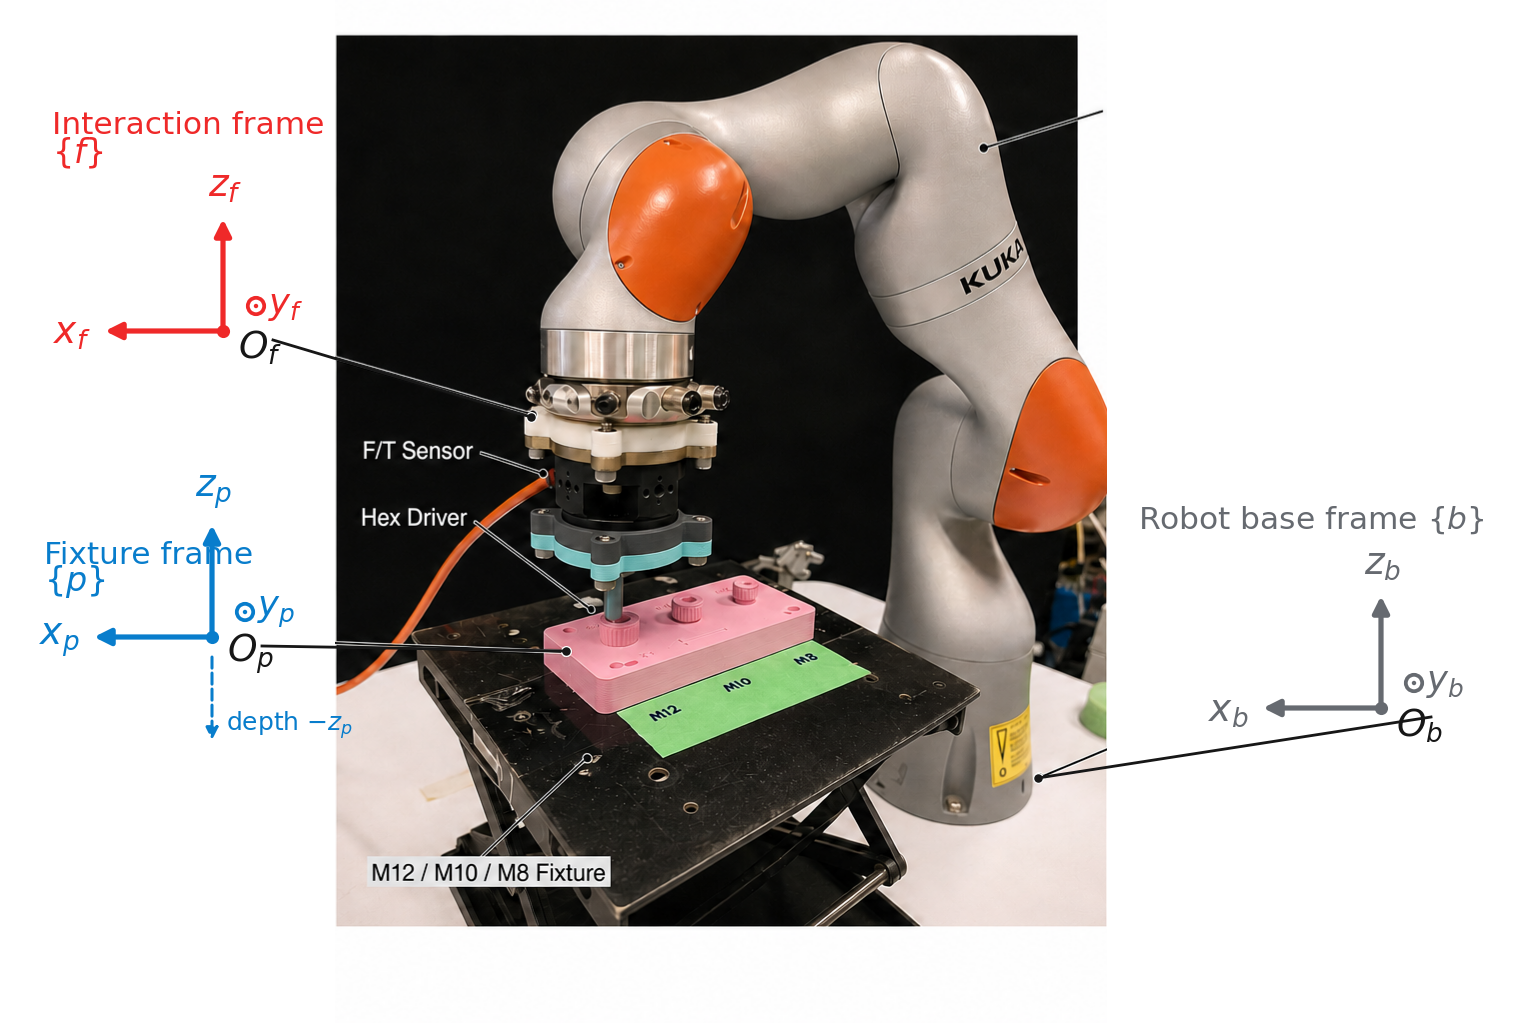
\includegraphics[width=0.80\textwidth]{figures/fig1_hardware_coordinate_frames.png}
  \caption{Experimental platform and coordinate-frame convention.  Frame
  $\{f\}$ sits on the force--torque-sensor/tool stack.  Frame $\{p\}$ sits
  on the M12/M10/M8 socket plate.  Frame $\{b\}$ sits on the KUKA LBR iiwa.
  All $z$ axes point up.  Engagement depth is measured along $-z_p$.  The
  $\odot$ marks show $y$ axes pointing out of the page.}
  \label{fig:hardware_frames}
\end{figure*}

The conical probe gives a circular estimate over direction and contact
state.  It reweights a rough planar estimate instead of pinning down one
socket center.  The robot moves only as far as a safe, supported quantile,
then searches the rest locally.  Wrench limits, recovery, and the final
check stay the same no matter what the model predicts.  A shaky tactile
estimate can shorten the route.  It can never sign off on its own success.

The main contributions are as follows:
\begin{enumerate}
  \item extracting a phase-indexed tactile signal that gives direction and
  contact support from one low-force conical touch, while keeping the
  direction--distance ambiguity of the socket center in plain view;
  \item turning that signal into action: a risk-bounded shortcut plus a
  finite local search, both run through one shared compliant capture and
  recovery controller;
  \item testing this in a paired study that checks engagement, task-level
  efficiency, direct-ray accuracy, recovery, and transfer across sizes, and
  then running it on real hardware.
\end{enumerate}

The study stops at verified socket engagement.  Turning the screw,
releasing the thread, and extracting it are not part of this work.

%%%%%%%%%%%%%%%%%%%%%%%%%%%%%%%%%%%%%%%%%%%%%%%%%%%%%%%%%%%%%%%%%%%%%%%%%%%%%%%%
\section{Problem Formulation}

\subsection{Task and observations}

Let $\{b\}$, $\{p\}$, and $\{f\}$ be the robot-base, fixture, and
interaction frames in Fig.~\ref{fig:hardware_frames}.  All planar
quantities below are written in $\{p\}$.  Here $C\in\R^2$ is the unknown
socket center.  $x_0\in\R^2$ is the tool position at the first stable top
contact.  $p_0(C)$ is a truncated visual/CAD prior over a finite set $G$.
During interaction, the controller reads robot pose and the wrench
\begin{equation}
w=[F_x,F_y,F_z,\tau_x,\tau_y,\tau_z]^\top .
\label{eq:wrench}
\end{equation}
The true center and contact labels from simulation are held back, for
offline checking only.

From the stable top contact, the tool runs a $15^\circ$ low-force conical
motion.  With phase $\phi$, the observation is resampled into
\begin{equation}
y(\phi)=
\begin{bmatrix}
F_z(\phi)&\tau_x(\phi)&\tau_y(\phi)&z_{\rm tip}(\phi)
\end{bmatrix}^{\!\top},
\quad \phi\in[0,2\pi).
\label{eq:fingerprint}
\end{equation}
Note that probe phase $\phi$ is not the planar direction angle $\theta$
from $x_0$ to $C$.  Those are two different things.  The height channel
records what comes with the wrench signal.  It is not an insertion
detector.  For each channel $c$, the samples are ordered on the circle and
linearly interpolated with periodic boundary conditions,
\begin{equation}
\begin{aligned}
\phi_n&=\frac{2\pi n}{N_\phi},\qquad n=0,\ldots,N_\phi-1,\\
y_c[n]&=\mathcal I_{\mathbb S^1}\{y_c\}(\phi_n),\qquad N_\phi=360.
\end{aligned}
\label{eq:phase_resampling}
\end{equation}
Here $\mathcal I_{\mathbb S^1}$ is the periodic interpolant.  This step
only fixes the input format.  It does not smooth the raw signal.

A trial counts as successful only if sensor-side capture is followed by a
steady bottom-mode dwell before $T_{\max}=130$~s, and only if no
force-limit stop happens first.  This verified-engagement event is the main
outcome we track.  We also report completion time $T_{\rm eng}$, measured
planar path $L_{xy}$, and a contact-work proxy $E_w$, all as conditional
efficiency measures.  Peak wrench and the exit reason are kept too, to help
read failures.  Let $\gamma_{\rm cap}$, $\gamma_{\rm bot}$, and
$\gamma_{\rm safe}$ be the capture, bottom-mode, and safety predicates.
The success event is then:
\begin{equation}
\begin{aligned}
\gamma_{\rm dwell}(t)&=\ind\!\left[
\int_{t-\Delta_b}^{t}\gamma_{\rm bot}(s)\,ds=\Delta_b\right],\\
\gamma_{\rm safe}^{[0,t]}&=\min_{s\in[0,t]}\gamma_{\rm safe}(s),\\
\mathcal V&=\{\exists\,t_c<t_b\le T_{\max}:\\
&\qquad\gamma_{\rm cap}(t_c)\gamma_{\rm dwell}(t_b)
\gamma_{\rm safe}^{[0,t_b]}=1\}.
\end{aligned}
\label{eq:verified_event}
\end{equation}
For a verified trial that starts at stable touchdown $t_0$, we report
\begin{align}
T_{\rm eng}&=t_b-t_0,\qquad
L_{xy}=\int_{t_0}^{t_b}\|\dot x(t)\|_2\,dt,
\nonumber\\
E_w&=\int_{t_0}^{t_b}\left(
|F_{xy}^{\top}\dot x|+|\tau^{\top}\omega|\right)dt .
\label{eq:hardware_metrics}
\end{align}

\subsection{Direction--distance ambiguity}

Let $r=\|C-x_0\|$.  Let the circular distance be
\begin{equation}
\dS(a,b)=\left|\operatorname{atan2}\!\left(\sin(a-b),\cos(a-b)\right)\right|\in[0,\pi].
\label{eq:circular_distance}
\end{equation}
Then $\epsilon=\dS(\hat\theta,\theta^\star)$ is the circular error of a
direct ray.  Under ideal planar motion, the closest gap between that ray
and the socket center is
\begin{equation}
d_\perp=r|\sin\epsilon|,\qquad
d_\parallel=r\cos\epsilon .
\label{eq:direct_miss}
\end{equation}
Here $r_{\rm eff}$ is a safe planar capture radius.  It is fixed per socket
size from the hex clearance, the chamfer shape, and how much slack the
compliant contact allows.  The ray only hits the capture disk if
$d_\perp\le r_{\rm eff}$ and $d_\parallel>0$.  So a small angle error is
harmless near the center.  Far from the center, the same small error can
miss completely.  The conical scan never sees $r$, so a direction estimate
alone cannot pick a safe endpoint.  Differently, in this work, we use two
steps instead: touch first updates a planar center belief, and only then
does it decide how far to travel.

%%%%%%%%%%%%%%%%%%%%%%%%%%%%%%%%%%%%%%%%%%%%%%%%%%%%%%%%%%%%%%%%%%%%%%%%%%%%%%%%
\section{Tactile Posterior-Guided Control Framework}

Figure~\ref{fig:framework} splits the system into two parts: learned
tactile inference and belief-space routing on one side, physical
interaction control on the other.  Blue blocks pull contact-state and
direction estimates out of the conical touch.  Green blocks then mix that
estimate with CAD support, and set a capped shortcut plus a residual
search.  A shortcut that misses is itself useful: it becomes negative
evidence before the residual route runs.  Below the authority line, the
black loop drives the robot--socket contact.  The red loop sits apart from
it and keeps the recovery and terminal calls.

\begin{figure*}[t]
  \centering
  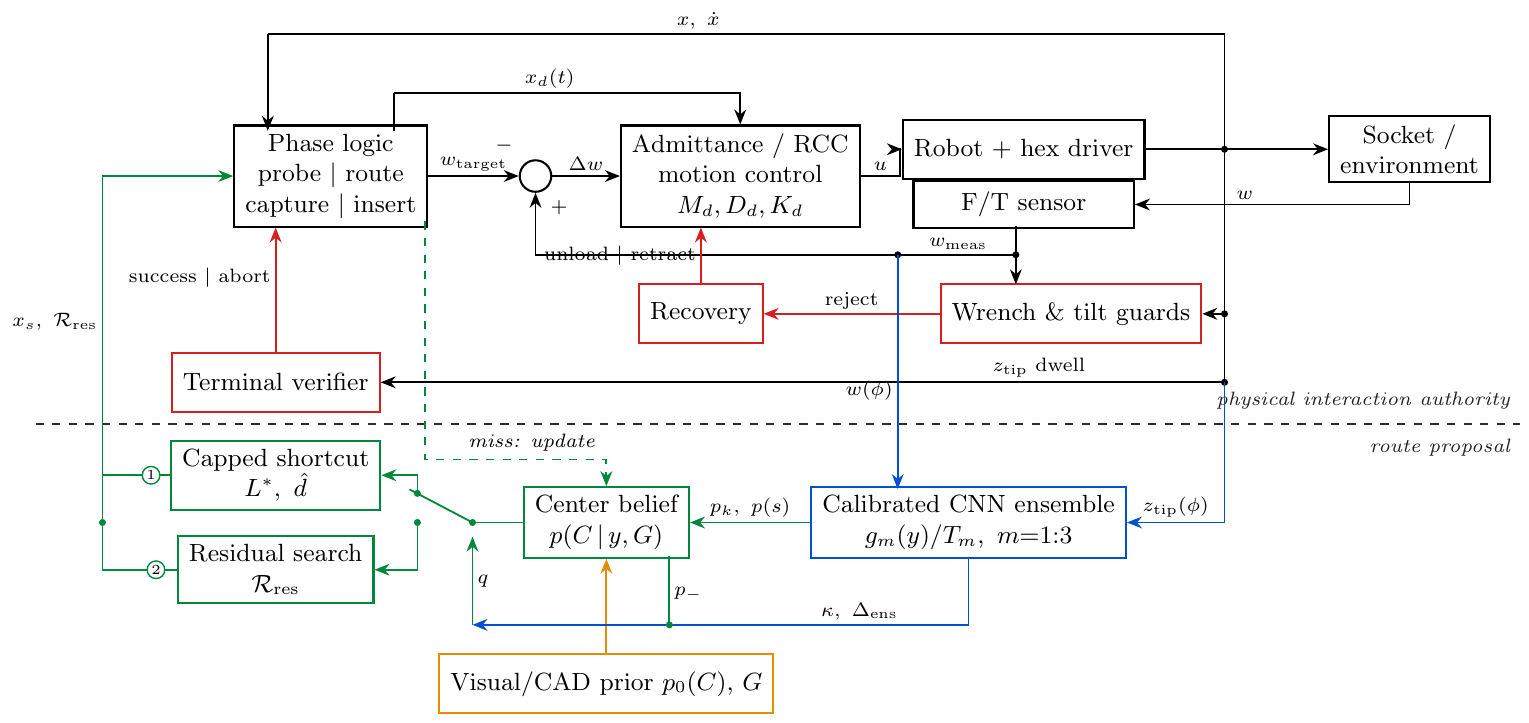
\includegraphics[width=0.98\textwidth]{figures/fig2_control_framework.png}
  \caption{Control architecture of the proposed framework.  Blue blocks are
  learning-based tactile inference.  Orange is the visual/CAD prior.  Green
  is the center-belief and task-planning path.  Black is the physical
  control loop.  Red is the wrench, recovery, and terminal guards.  The
  dashed line separates route proposals from physical control.}
  \label{fig:framework}
\end{figure*}

\subsection{Circular tactile posterior}

Three separately trained models map the $4\times360$ signal to logits over
$K=48$ direction bins.  After temperature calibration, their average is
\begin{equation}
p_k=\frac{1}{M}\sum_{m=1}^{M}
\softmax\!\left(\frac{g_m(y)}{T_m}\right)_k,
\qquad M=3.
\label{eq:ensemble}
\end{equation}
Its circular mean and concentration are
\begin{align}
\mu&=\arg\sum_k p_ke^{i\theta_k},\qquad
\kappa=\left|\sum_k p_ke^{i\theta_k}\right|,
\nonumber\\
\hat d&=[\cos\mu,\sin\mu]^\top .
\label{eq:circular_stats}
\end{align}
A second head gives a rough contact-support score $p(s)$.  An adaptive
prediction set~\cite{romano2020aps} sums up angular support.  Separately,
the largest top-1 gap $\Delta_{\rm ens}$ across ensemble members marks how
much the models disagree.  These are only descriptions of the observation.
None of them counts as capture.  More precisely, order the bins so that
$p_{\pi(1)}\ge\cdots\ge p_{\pi(K)}$.  At kept mass $1-\eta$, the set used
is
\begin{align}
r_\eta&=\min\left\{r:\sum_{\ell=1}^{r}p_{\pi(\ell)}\ge1-\eta\right\},
\nonumber\\
\mathcal A_\eta&=\{\pi(1),\ldots,\pi(r_\eta)\}.
\label{eq:aps_set}
\end{align}
Let $\hat\theta_m=\theta_{\arg\max_k p_{m,k}}$ be the top bin of member
$m$.  The disagreement across the ensemble is then
\begin{equation}
\Delta_{\rm ens}=\max_{m,n\in\{1,\ldots,M\}}
\dS(\hat\theta_m,\hat\theta_n).
\label{eq:ensemble_disagreement}
\end{equation}
We also keep the entropy of the posterior, in nats, as one more check on
how spread out it is,
\begin{equation}
H(p)=-\sum_{k=1}^{K}p_k\log p_k,
\label{eq:posterior_entropy}
\end{equation}
A tight posterior can still hide members that disagree.  A spread-out
posterior can still hide members that agree.  These are not the same thing,
so we keep both numbers.  Figure~\ref{fig:fingerprint} shows the whole
chain.  Real keyframes show the conical motion as run on hardware.  One
held-out MuJoCo record then shows the raw signal, the posterior, and the
route it produces.

\begin{figure*}[t]
  \centering
  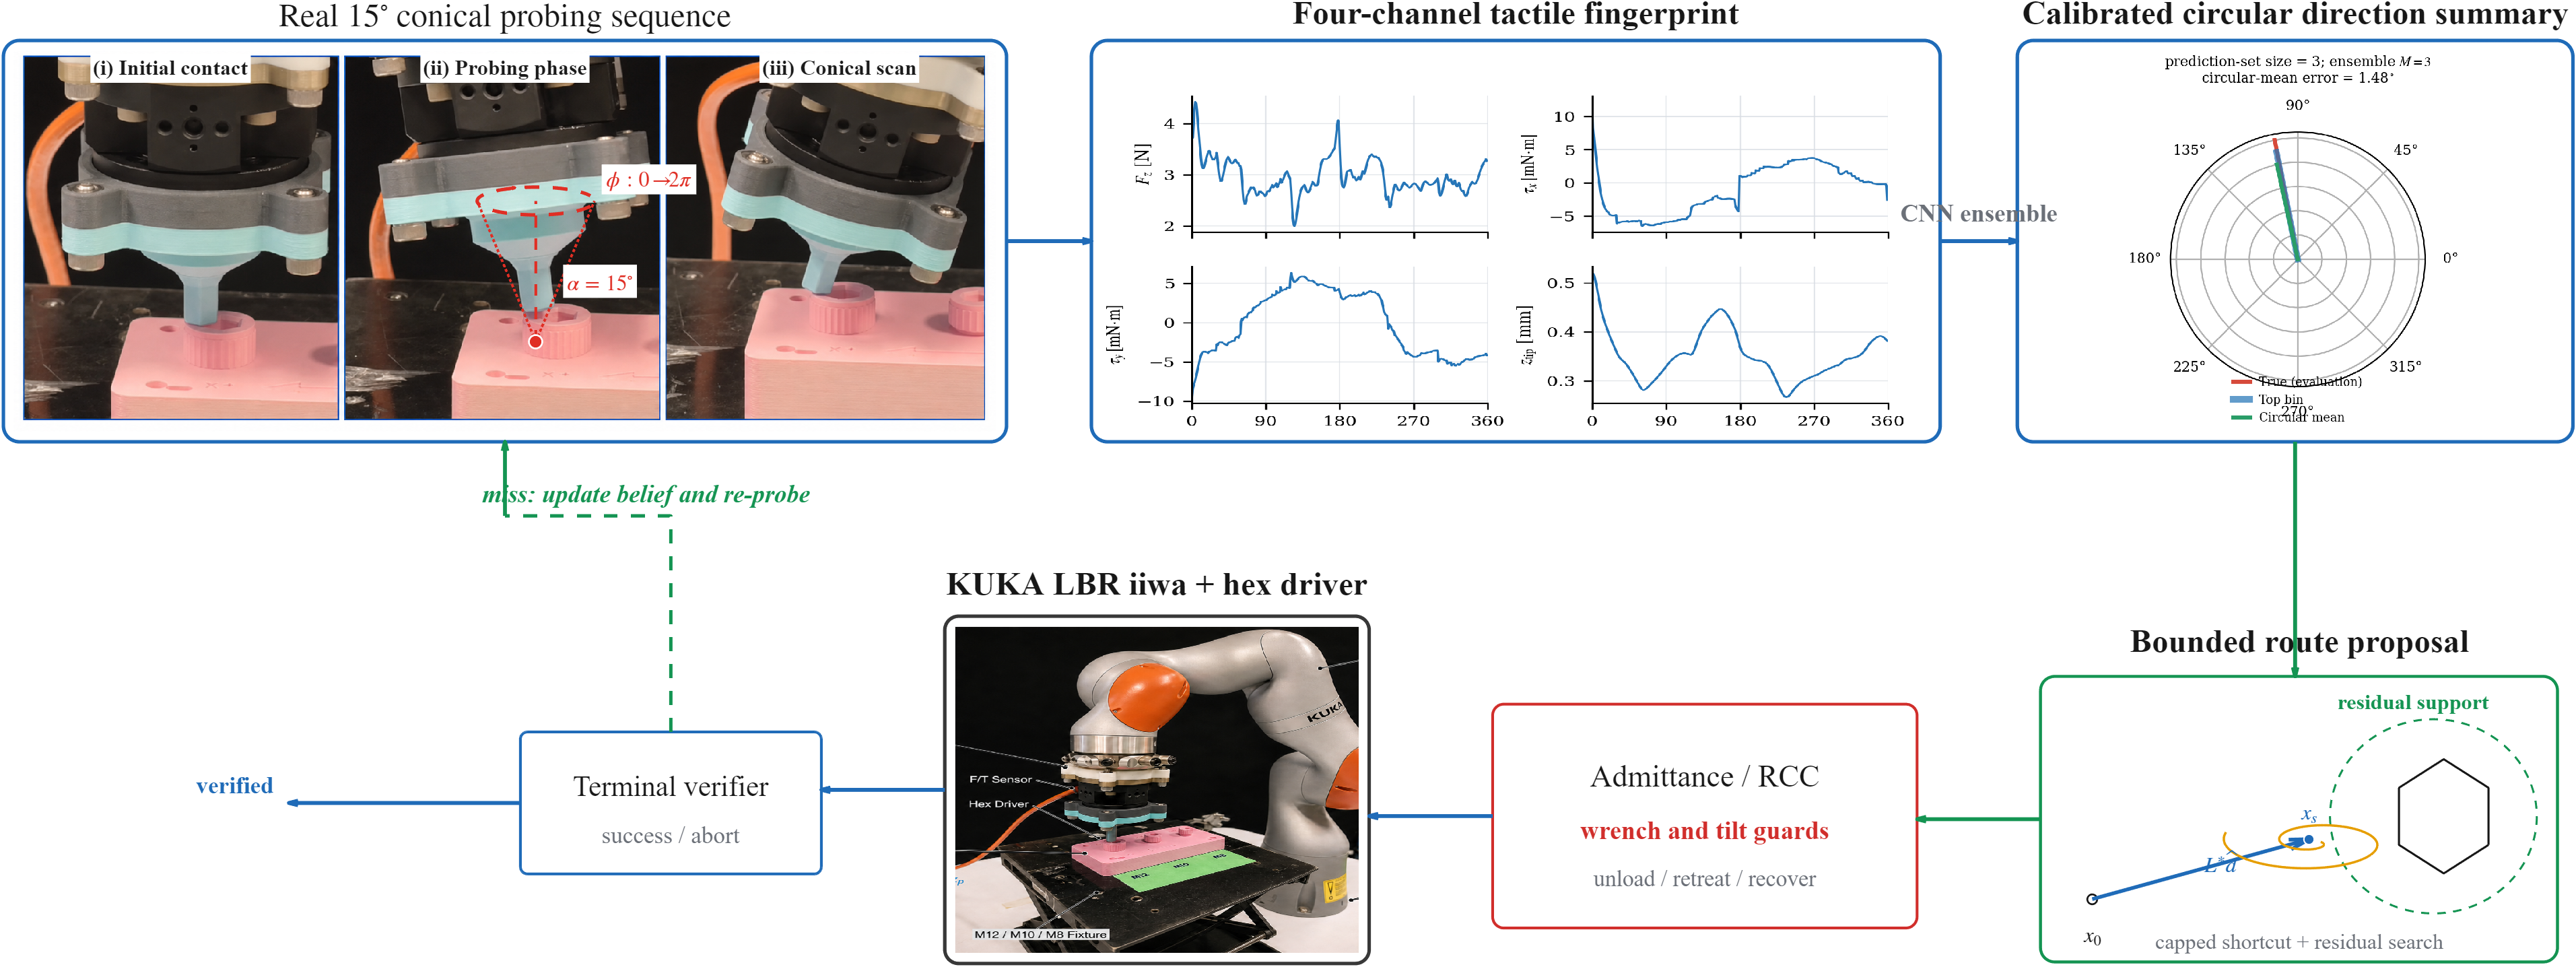
\includegraphics[width=0.98\textwidth]{figures/fig3_action_observation_routing.png}
  \caption{Closed-loop tactile-guided search.  Real keyframes show first
  contact, probing, and the $15^\circ$ conical scan.  A held-out MuJoCo
  example shows the four-channel signal and the circular summary built from
  it (three-bin prediction set, ensemble size $M=3$, circular-mean error
  $1.48^\circ$).  Direction and confidence set the shortcut and the
  residual route.  Admittance/RCC, wrench and tilt guards, and the final
  check stay in charge the whole time.  A miss updates the belief before
  the next probe.}
  \label{fig:fingerprint}
\end{figure*}

\subsection{From tactile direction to center belief}

The visual prior is a set of $N=4096$ center particles,
\begin{equation}
C_j=x_0+\delta_j,\qquad
\delta_j\sim\mathcal N(0,\sigma_v^2I)\mid\|\delta_j\|\le R_v .
\label{eq:center_samples}
\end{equation}
For M8, $\sigma_v=2$~mm and $R_v=4.895$~mm.  Each particle gets a new
weight, from the posterior probability of its angular bin times a radial
likelihood $L_s$ tied to contact support:
\begin{equation}
\bar w_j=\frac{p_{b(\arg\delta_j)}
\left[0.02+0.98\sum_s p(s)L_s(\|\delta_j\|)\right]}
{\sum_\ell p_{b(\arg\delta_\ell)}
\left[0.02+0.98\sum_s p(s)L_s(\|\delta_\ell\|)\right]}.
\label{eq:center_weights}
\end{equation}
The small uniform term stops one shaky reading from erasing the geometric
support.  More to the point, it keeps the radial ambiguity in plain view,
instead of burying it inside a point estimate.  For later use, the weighted
empirical quantile is
\begin{equation}
Q_\rho^w(a)=\inf\left\{u:\sum_{j=1}^{N}\bar w_j\ind[a_j\le u]\ge\rho\right\}.
\label{eq:weighted_quantile}
\end{equation}

\subsection{Risk-bounded shortcut and residual search}

Project each particle onto the estimated ray, $z_j=(C_j-x_0)^\top\hat d$.
Call $p_-=\sum_j\bar w_j\ind[z_j\le0]$ the posterior mass sitting behind
the current contact.  Observation quality is then
\begin{align}
q&=\clip\!\left(\kappa[\cos(\Delta_{\rm ens}/2)]_+(1-2p_-),0,1\right),
\nonumber\\
\alpha(q)&=0.10+0.15q,\qquad
\lambda(q)=0.35+0.30q .
\label{eq:shortcut_quality}
\end{align}
So evidence that is spread out, disagreeing, or pointing backward earns
less direct travel.

Let $Q_\rho^w(\cdot)$ be a weighted empirical quantile, and $L_c$ an
optional command cap.  The allowed shortcut is then
\begin{align}
L_{\rm proj}&=[Q_{\alpha(q)}^w(z)-0.25r_{\rm eff}]_+,
\nonumber\\
L_{\rm rad}&=\lambda(q)Q_{0.99}^w(\|C-x_0\|),
\nonumber\\
L^*&=
\begin{cases}
0,&p_-\ge0.20,\\
\min\{L_{\rm proj},L_{\rm rad},L_c\},&p_-<0.20,
\end{cases}
\nonumber\\
x_s&=x_0+L^*\hat d .
\label{eq:shortcut_length}
\end{align}

\begin{proposition}[Posterior mass retention]
Assume $p_-<0.20$, $L^*>0$, and that the shortcut endpoint is reached
exactly.  For a fixed weighted-particle set, the shortcut obeys
\begin{align}
\widehat{\mathbb P}_w[z\ge L^*+0.25r_{\rm eff}]&\ge1-\alpha(q),
\nonumber\\
L^*&\le\lambda(q)Q_{0.99}^w(\|C-x_0\|).
\label{eq:shortcut_bound}
\end{align}
\end{proposition}
\begin{proof}
Take $L^*>0$.  Then $L^*\le L_{\rm proj}$, so $L^*+0.25r_{\rm eff}\le
Q_{\alpha(q)}^w(z)$.  By how the weighted quantile is built, at least
$1-\alpha(q)$ of the empirical mass sits at or above that point.  That is
the first bound.  We also have $L^*\le L_{\rm rad}$.  The second bound
follows the same way.
\end{proof}

This result only allocates posterior support.  It does not promise capture.
The residual search radius after the shortcut is
\begin{equation}
R_{\rm res}=
\left[Q_{0.99}^w(\|C-x_s\|)-r_{\rm eff}\right]_+ .
\label{eq:residual_radius}
\end{equation}
Figure~\ref{fig:shortcut} shows this split.  In the case shown, a clear
reading allows 2.873~mm of direct travel and leaves a 1.732~mm local search
region.

\begin{figure*}[t]
  \centering
  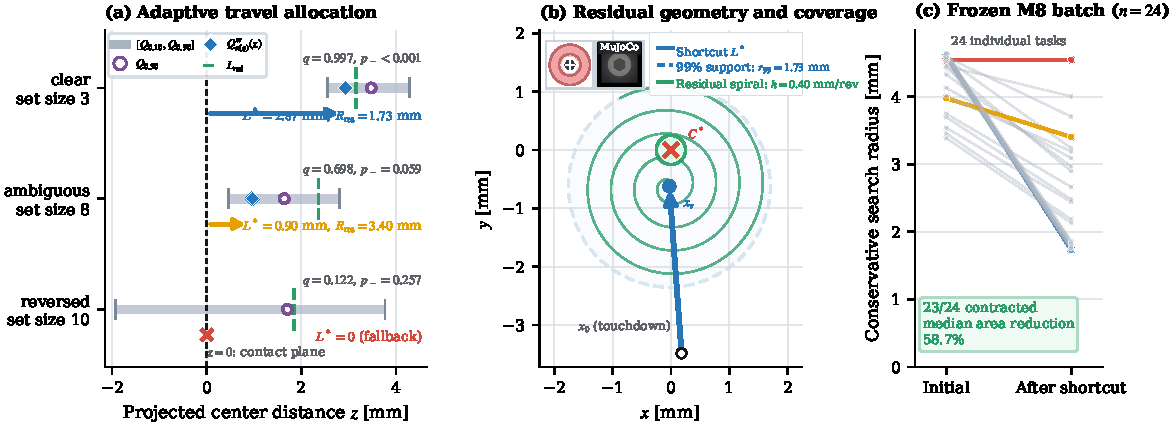
\includegraphics[width=0.96\textwidth]{figures/posterior_shortcut_geometry.pdf}
  \caption{Quality-adaptive posterior budgeting and residual search.
  (a) Three frozen M8 cases.  Direction quality and reverse posterior mass
  set the allowed travel, including the $L^*=0$ fallback.  Prediction-set
  size is 3, 8, and 10 bins in these cases.  (That is not the same number
  as the ensemble size, $M=3$.)  (b) The clear-observation command stops at
  a bounded endpoint (blue arrow).  The dashed disk is the remaining
  weighted 99\% radial envelope, and the green curve is the finite local
  spiral.  The centered-socket and MuJoCo insets
  are not to scale.  (c) How the conservative search disk shrinks, paired
  across all 24 frozen M8 tasks, with the three cases from (a) marked.
  Ground-truth center and capture-set marks are shown only for grading.
  The controller never sees them.  All quantitative marks come from trial
  records.}
  \label{fig:shortcut}
\end{figure*}

The measured shortcut is also a plain physical observation.  For an
executed move $a:x\rightarrow x_a$, let $d_a(C)$ be the shortest planar gap
from $C$ to that move.  The runtime uses a smooth capture likelihood,
\begin{align}
d_a(C)&=\min_{s\in[0,1]}\|C-[x+s(x_a-x)]\|_2,
\nonumber\\
\ell_{\rm cap}(C\mid a)&=\varepsilon_\ell+(1-2\varepsilon_\ell)
\sigma\!\left(\frac{r_{\rm eff}-d_a(C)}{h_\ell}\right),
\label{eq:segment_likelihood}
\end{align}
Here $h_\ell$ sets the width of the contact boundary, and
$\varepsilon_\ell$ keeps particles from dying out completely.  When the
measured endpoint is valid and still in guarded contact, but capture is
rejected, weights update as
\begin{equation}
\bar w_j^{+}=\frac{\bar w_j^{-}
[1-\ell_{\rm cap}(C_j\mid a)]}
{\sum_{\ell=1}^{N}\bar w_\ell^{-}
[1-\ell_{\rm cap}(C_\ell\mid a)]}.
\label{eq:miss_update}
\end{equation}
The residual geometry is then rebuilt around the measured endpoint.  An
endpoint that is invalid or never observed does not trigger this update.

The \pgso{} variant covers the residual region with a finite local
Archimedean spiral, pitch $h_{\rm sp}$,
\begin{equation}
\begin{aligned}
x_{\rm sp}(\psi)&=x_s+\frac{h_{\rm sp}\psi}{2\pi}
\begin{bmatrix}\cos\psi&\sin\psi\end{bmatrix}^{\!\top},\\
0&\le\psi\le\frac{2\pi R_{\rm res}}{h_{\rm sp}}.
\end{aligned}
\label{eq:residual_spiral}
\end{equation}
The \pgsg{} variant instead scores each candidate move
$a:x\rightarrow x_a$ by
\begin{align}
U(a)={}&\beta_I I(C;O\mid a)
+\beta_P\widehat{\mathbb P}_w([x,x_a]\cap B_{r_{\rm eff}}(C)\ne\varnothing)
\nonumber\\[-1mm]
&-c_0-c_\ell\|x_a-x\| .
\label{eq:grid_utility}
\end{align}
The first term rewards a contact that tells the most.  The second rewards a
move that covers likely capture disks.  The last terms simply tax switching
and travel.  When further contact stops being useful, the planner falls
back to plain coverage.  It does not force entropy to keep dropping.  For
the binary outcome $O\in\{\mathrm{hit},\mathrm{miss}\}$, the information
gain in~\eqref{eq:grid_utility} works out to
\begin{equation}
I(C;O\mid a)=H(\bar w)-
\sum_{o\in\{\mathrm{hit},\mathrm{miss}\}}
P(o\mid a)H(\bar w\mid o,a),
\label{eq:expected_information_gain}
\end{equation}
and the next move is picked only from what is left of the action set
$\mathcal A_{\rm rem}$:
\begin{equation}
a^*=\arg\max_{a\in\mathcal A_{\rm rem}}U(a).
\label{eq:grid_action_selection}
\end{equation}

\subsection{Compliant capture, recovery, and verification}

Every search policy shares the same task-frame admittance/RCC controller,
\begin{equation}
M_d\ddot\xi+D_d\dot\xi+K_d\xi=w_{\rm meas}-w_{\rm target},
\label{eq:admittance}
\end{equation}
plus rate saturation and a causal first-order wrench filter,
\begin{align}
\alpha_f&=\frac{\Delta t}{(2\pi f_c)^{-1}+\Delta t},
\nonumber\\
\bar w_t&=\bar w_{t-1}+\alpha_f(w_t-\bar w_{t-1}).
\label{eq:wrench_filter}
\end{align}
Each wrench and tilt component is checked on its own,
\begin{equation}
\gamma_{\rm safe}(t)=
\ind\!\left[\left\|\bar w(t)\oslash w_{\max}\right\|_\infty\le1
\;\land\;|\alpha_{\rm tilt}(t)|\le\alpha_{\max}\right],
\label{eq:safety_guard}
\end{equation}
where $\oslash$ is elementwise division.  A capture cue only hands off to
an insertion attempt.  It does not force one.  If progress stalls or tilt
gets too large, the recovery operator kicks in:
\begin{equation}
\begin{aligned}
\mathcal R={}&\mathsf{retouch}_{0.20\,\mathrm{s}}\circ
\mathsf{upright}\\
&\circ\mathsf{retract}_{0.35\,\mathrm{mm},\,0.15\,\mathrm{s}}
\circ\mathsf{unload}_{0.10\,\mathrm{s}}.
\end{aligned}
\label{eq:recovery_map}
\end{equation}
It picks up from the measured state.  At most three recoveries are
allowed.  With axial progress $d(t)=z_{\rm tip}(t_0)-z_{\rm tip}(t)$, the
bottom and terminal predicates are
\begin{align}
\gamma_{\rm bot}(t)&=\ind[d(t)\ge d_{\rm req}-\varepsilon_d],
\nonumber\\
\gamma_{\rm term}(t)&=\gamma_{\rm safe}(t)
\ind\!\left[\int_{t-\Delta_b}^{t}\gamma_{\rm bot}(s)\,ds=\Delta_b\right].
\label{eq:terminal_dwell}
\end{align}
Here $\varepsilon_d$ is the registered terminal-depth tolerance.
Engagement is accepted only once this independent dwell holds.  A
force-limit hit, or a budget that runs out, ends the trial instead.

%%%%%%%%%%%%%%%%%%%%%%%%%%%%%%%%%%%%%%%%%%%%%%%%%%%%%%%%%%%%%%%%%%%%%%%%%%%%%%%%
\section{Experiments}

\subsection{Setup, baselines, and measures}

The main simulation benchmark has 24 task tuples, fixed before any policy
is compared.  A Sobol design varies planar offset, socket phase, sliding
friction, contact dynamics, target force, sensing delay, and the
posterior/noise seeds, all together.  Radial offset spans 1.74--4.88~mm,
sliding friction 0.564--0.945, contact time constant 40.6--69.7~ms,
sensing delay 2.00--7.87~ms, and target downward force 2.50--3.44~N.
Every policy gets the same tuple, the same 130~s budget, the same capture
controller, and the same terminal check.  No simulator reset and no budget
extension is allowed.

Four task-level policies are compared.  (i) \pgso{} uses the posterior
shortcut, then an outward residual spiral.  (ii) \pgsg{} keeps the shortcut
but swaps the residual for an entropy grid, which picks the next low-force
contact from expected information gain and coverage.  (iii) \emph{Outward}
runs a plain global Archimedean search, with no tactile shortcut at all.
(iv) \emph{Direct-4C} spends up to three physical rays along directions
read off the four-channel signal.  A missed direct ray unloads, shifts
0.25~mm across the ray, and repeats the full probe in the same rollout.

A second direct arm, \emph{Direct-3C}, is used only for a representation
check.  It swaps $[F_z,\tau_x,\tau_y,z_{\rm tip}]$ for the three polar
channels $[x_z,M_x,M_y]$ plus a 12-sector decision, following the
contact-pose idea in~\cite{jin2021contact}.  This is our own proxy built
for the same task.  It is not a copy of that reference controller.  Recent
force-guided and belief-space exploration
work~\cite{noseworthy2025forge,chintalapudi2026bilevel} matters for
context.  We do not give it a quantitative row, though, since its sensing,
action, and terminal rules are not reproduced here.

Completion time stops at the verified terminal dwell.  Planar path is the
integral of measured tip motion.  A force-limit stop, a protected
post-capture stop, or running out of search budget all count as failure.
Medians inside the successful group are only descriptive.  Efficiency
claims instead come from paired differences across joint completions, and
binary recovery comparisons use exact paired tests.  Every curve we show is
rebuilt from frozen per-trial simulator records or timestamped hardware
logs.  No series is interpolated, smoothed, or filled in.  The only changes
made are the stated frame changes, same-run baseline subtraction, grouping,
and cumulative counting.

\subsection{Four-channel tactile representation}

This check holds the first conical touch, the task tuple, the noise seed,
the direct-ray budget, and the post-capture controller all fixed.  So it
asks a narrower question than the full policy comparison: does adding the
height channel and the circular posterior change the direction the
controller actually uses?  Figure~\ref{fig:representation} shows the full
paired set plus one audited example.  Direct-4C has a smaller median error.
Its tail is heavier, though, so we cannot call it uniformly more accurate.

\begin{figure*}[t]
  \centering
  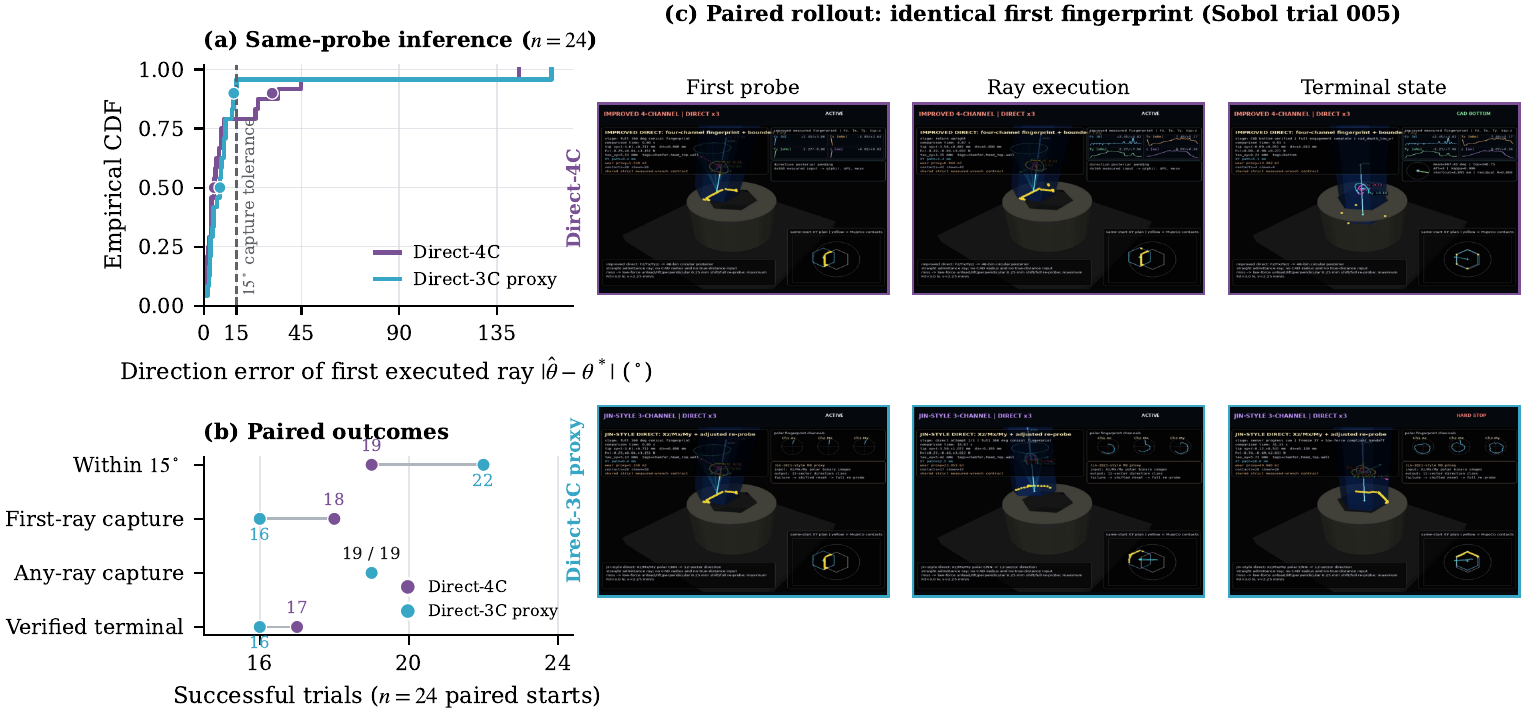
\includegraphics[width=0.98\textwidth]{figures/m8_four_channel_representation_ablation.png}
  \caption{Controlled tactile-representation ablation.  (a) Empirical CDF
  of the first direction the controller actually runs, on all 24 paired M8
  starts.  Circles mark the median and the 90th percentile.  (b) Paired
  capture and terminal counts.  (c) Frames from Sobol 005, same raw
  fingerprint for both methods.  Direct-4C captures on its first ray and
  reaches the terminal set.  The three-channel proxy instead pays for three
  full probes, hands off to the shared capture controller on the third try,
  and then exits at a wrench limit.  Direct-4C is the proposed
  representation.  Direct-3C is the three-channel proxy.  Panel (c) is one
  case, not a ranking across the population.}
  \label{fig:representation}
\end{figure*}

\begin{table}[t]
\caption{Same-probe direct-ray ablation on 24 paired M8 starts.  Exact
McNemar values apply only to the binary paired outcomes.}
\label{tab:direct}
\centering
\scriptsize
\setlength{\tabcolsep}{3.4pt}
\begin{tabular}{lccc}
\toprule
Measure & Direct-4C & Direct-3C & Paired $p$\\
\midrule
Median error & $4.75^\circ$ & $7.41^\circ$ & --\\
90th-percentile error & $31.45^\circ$ & $13.79^\circ$ & --\\
Within $15^\circ$ & 19/24 & 22/24 & 0.375\\
First-ray capture & 18/24 & 16/24 & 0.6875\\
Any-ray capture, $\le3$ & 19/24 & 19/24 & 1.0\\
Verified terminal & 17/24 & 16/24 & 1.0\\
\bottomrule
\end{tabular}
\end{table}

The result here is deliberately mixed.  The fourth channel tightens the
central error and adds two first-ray captures.  The sectorized proxy, on
the other hand, gets the smaller 90th-percentile error and three more cases
within $15^\circ$.  The any-ray capture count ties, and the terminal gap is
only one trial (Table~\ref{tab:direct}).  So we keep the four-channel
signal because it feeds the shortcut and the entropy grid, not because this
one batch proves it always points better.

\subsection{Paired M8 closed-loop search}

Figure~\ref{fig:policy_sequence} shows how the four policies use the same
muted first contact in Sobol 016.  (i) \pgsg{} spends the weak direction
cue on a short move, then picks residual contacts from the entropy grid.
(ii) \pgso{} follows with an outward residual spiral.  (iii) Outward pays
for full coverage from the same starting contact.  (iv) Direct-4C uses up
its three physical rays.  Frames are lined up by progress within each
policy, so each row stays in order.  What decides efficiency is the raw
time and path, not how the frames happen to be spaced on the page.

\begin{figure*}[t]
  \centering
  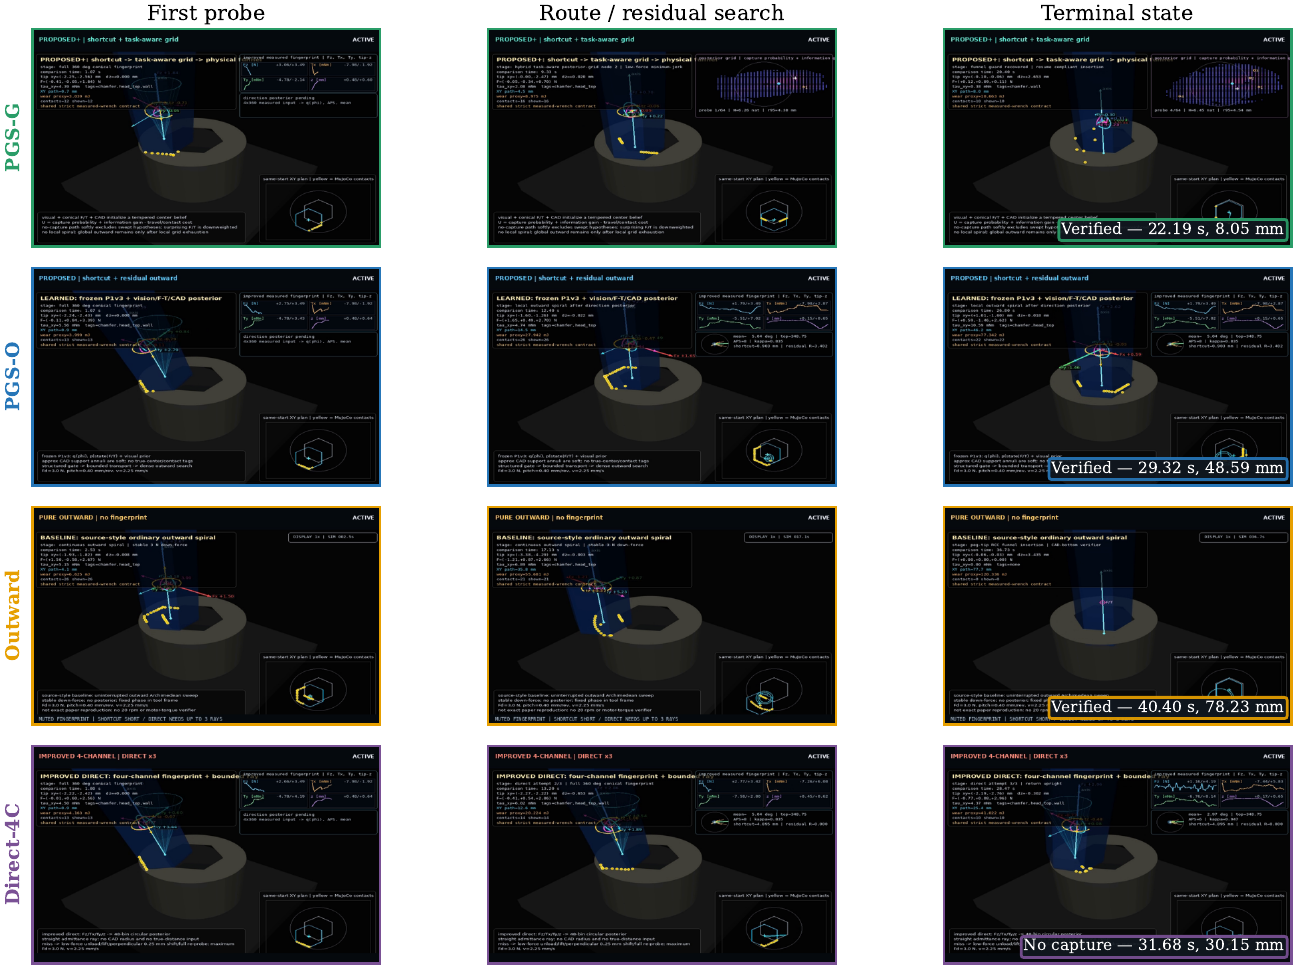
\includegraphics[width=0.98\textwidth]{figures/m8_four_policy_keyframe_matrix.png}
  \caption{Chronological MuJoCo keyframes, one muted-fingerprint M8 case
  (Sobol 016).  Rows: \pgsg{}, \pgso{}, Outward, Direct-4C.  Columns: early
  probe, route/residual search, terminal state.  Yellow points mark
  measured contacts.  Each inset is the task-plane trace from that same
  start.  \pgsg{}, \pgso{}, and Outward all reach CAD-bottom verification.
  Direct-4C runs out of its ray budget first, with no capture.  Badges show
  values from this one frozen trial.  They will not match the medians in
  Table~\ref{tab:m8_results}.}
  \label{fig:policy_sequence}
\end{figure*}

Figure~\ref{fig:summary} and Table~\ref{tab:m8_results} cover the full
paired set.  The question the curves answer is simple: given a fixed time
or a fixed distance, how many paired tasks have already engaged?  \pgso{}
gets there in 20/24 cases.  \pgsg{} and Outward tie at 19/24.  Direct-4C
often finishes fast, when its estimated ray happens to land in the capture
region, but it settles at a lower total.

\begin{figure*}[t]
  \centering
  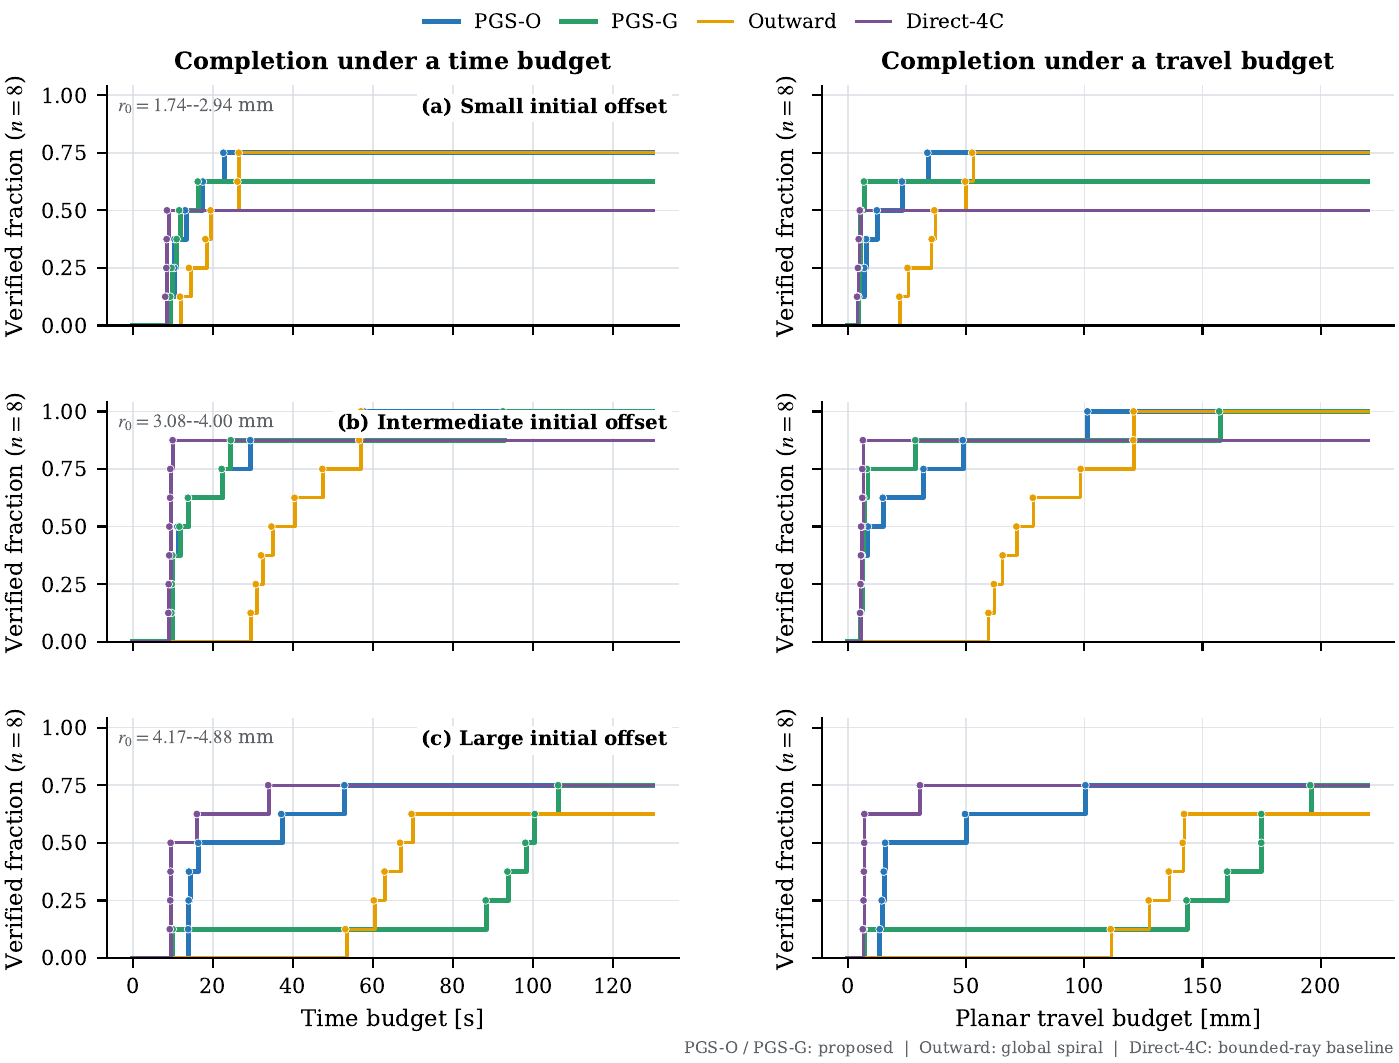
\includegraphics[width=0.96\textwidth]{figures/m8_budgeted_engagement_profiles.png}
  \caption{Budgeted M8 engagement, 24 paired starts, split into three
  equal-size offset groups: (a) small, (b) medium, (c) large.  Left column:
  fraction of eight tasks done within a time budget.  Right column: same,
  using measured planar travel as the budget.  Each row has $n=8$ trials.
  The ordinate is the fraction that has reached verified engagement.  Step
  points mark recorded terminal times and travel distances.  Nothing here
  is smoothed or interpolated.  A failed trial adds no step, so each
  plateau reflects both success and speed.}
  \label{fig:summary}
\end{figure*}

\begin{table*}[t]
\caption{M8 engagement results on 24 paired starts.  $T_{\rm eng}$,
$L_{xy}$, and $E_w$ are medians over successful trials.  $\|F\|_{\max}$ is
the median trial maximum over all starts.  The last column lists hard-stop,
protected, and budget/radius exits ($H/P/B$).}
\label{tab:m8_results}
\centering
\footnotesize
\setlength{\tabcolsep}{6.2pt}
\begin{tabular}{lcccccc}
\toprule
Method & Verified & $T_{\rm eng}$ [s] & $L_{xy}$ [mm] & $E_w$ [mJ] & $\|F\|_{\max}$ [N] & $H/P/B$\\
\midrule
\pgso{} & \textbf{20/24} & 13.87 & 14.52 & 28.48 & 7.33 & 3/0/1\\
\pgsg{} & 19/24 & 13.74 & 6.76 & 9.54 & 7.69 & 4/0/1\\
Outward & 19/24 & 34.63 & 71.27 & 120.38 & 7.45 & 4/1/0\\
Direct-4C & 17/24 & 9.22 & 6.07 & 13.67 & 7.33 & 3/0/4\\
\bottomrule
\end{tabular}
\end{table*}

\subsection{Efficiency and component ablations}

\pgso{} and Outward both finish 19 trials.  On that shared subset, \pgso{}
covers less ground in 19 of 19, and takes less time in 18 of 19.  Median
paired gaps are $-41.14$~mm and $-16.79$~s, with exact sign-test values
$p=3.8\times10^{-6}$ and $p=7.6\times10^{-5}$.  This test compares the full
probe--shortcut--residual policy against plain global coverage.  On its
own, it does not pull the shortcut apart from every other choice in the
policy.

\pgsg{} and \pgso{} share 19 completions.  Median paired path gap:
$-0.061$~mm (11/19 shorter, Wilcoxon $p=0.465$).  Median paired time gap:
$+0.536$~s (7/19 faster, $p=0.196$).  In other words, the gain over Outward
cannot be pinned on the entropy grid.  In this benchmark, the residual
disks are only a few millimeters wide, so a local spiral already covers
them with little wasted motion.  The grid also scores contacts with the
same rough likelihood used for the belief update, and close candidate
scores, model error, plus the cost of unloading and touching again, can
easily erase a small geometric gain.  Bigger search regions or a
better-calibrated likelihood might change this.  The 24 starts here do not
show that advantage.

Recovery is checked on a separate, fixed 12-case post-capture stress set.
With the RCC and wrench guards left alone, turning recovery off gives no
verified engagement.  Allowing up to three recoveries gives 9/12, with no
case going the other way (exact two-sided $p=0.00390625$).  Two force-limit
exits and one protected exit remain.  Recovery changes what state is
reachable after a rejection.  It does not force a win.

\subsection{Cross-size simulation}

We next check whether this narrow learned interface transfers from M8 to
M10/M12, keeping the physical controller fixed.  For each size, 72
training, 36 validation, and 36 calibration scans are split by sixfold
symmetry.  The encoder stays fixed.  Only the contact-state and direction
heads get updated, with an $\ell_2$ anchor back to the M8 weights.  A
concentration and source-agreement gate turns off the shortcut when the
adapted head looks unsure.  Residual search and every physical guard stay
untouched.

\begin{table}[t]
\caption{Cross-size engagement ($n=12$ per cell): verified / force-limit /
protected termination.  Remaining trials end by budget or terminal rejection.}
\label{tab:cross_size}
\centering
\scriptsize
\setlength{\tabcolsep}{2.4pt}
\begin{tabular}{@{}lcccc@{}}
\toprule
Interface & Dev M10 & Dev M12 & Test M10 & Test M12\\
\midrule
M8 zero-shot & 12/0/0 & 10/1/1 & 12/0/0 & 10/0/1\\
Calibration only & 12/0/0 & 10/0/1 & 12/0/0 & 11/0/0\\
Anchored fine-tuning & 12/0/0 & 10/0/2 & 10/1/1 & 10/0/2\\
Privileged center & 12/0/0 & 11/0/1 & 12/0/0 & 12/0/0\\
\bottomrule
\end{tabular}
\end{table}

Table~\ref{tab:cross_size} shows no steady held-out gain from anchored
fine-tuning over zero-shot or calibration-only transfer, even though it
looks good on development data.  So we keep residual search and the contact
guards outside the transferred network, and fit the observation model again
once it is on real hardware.

\subsection{Hardware evaluation}

Hardware data came from the tool and fixture registered in place.  For each
of M8, M10, and M12, the campaign has 16 clean conical scans, four
development holdouts, four quarantined points, and two repeated sentinels.
All 78 scheduled traces passed the acquisition checks, but their
phase-aligned signals looked clearly different from the rendered ones.
Coulomb and stiction error, deformed printed parts, sensor bias,
fixture/TCP registration, and the gravity moment at the Bota sensor all add
up to this gap.  So the circular model used on the robot was fit again, on
signals from the installed stack.  These records carry the full hardware
effect.  They do not fix session drift, wear, temperature changes, or
shifts across socket size.  The M12 holdouts were already seen during
development, so we do not treat them as an untouched test set.

Selected M12 runs went through the whole sequence: guarded touchdown,
conical scan, bounded routing, capture re-check, staged insertion, and
terminal dwell.  Named \pgso{}, \pgsg{}, and Direct-4C runs all reached the
terminal event.  Outward went over the 130~s budget.  When the same run was
let continue past that limit, it engaged after about 395~s.  Two fixed-site
M10 \pgsg{} pilots also reached terminal depths of 4.834 and 4.726~mm.

Figure~\ref{fig:hardware} shows one named M12 \pgsg{} run, start to finish,
with no mixing of trials.  Its 240-sample real signal gave a 3.00~mm
shortcut.  The measured endpoint missed the command by 0.054~mm, and did
not capture.  That negative result then redirected the residual policy.
Capture came 42.45~s after touchdown.  The terminal candidate was logged at
116.63~s, with 5.792~mm of measured insertion depth.  These numbers
describe only that one run, not a general rate.

\begin{figure*}[t]
  \centering
  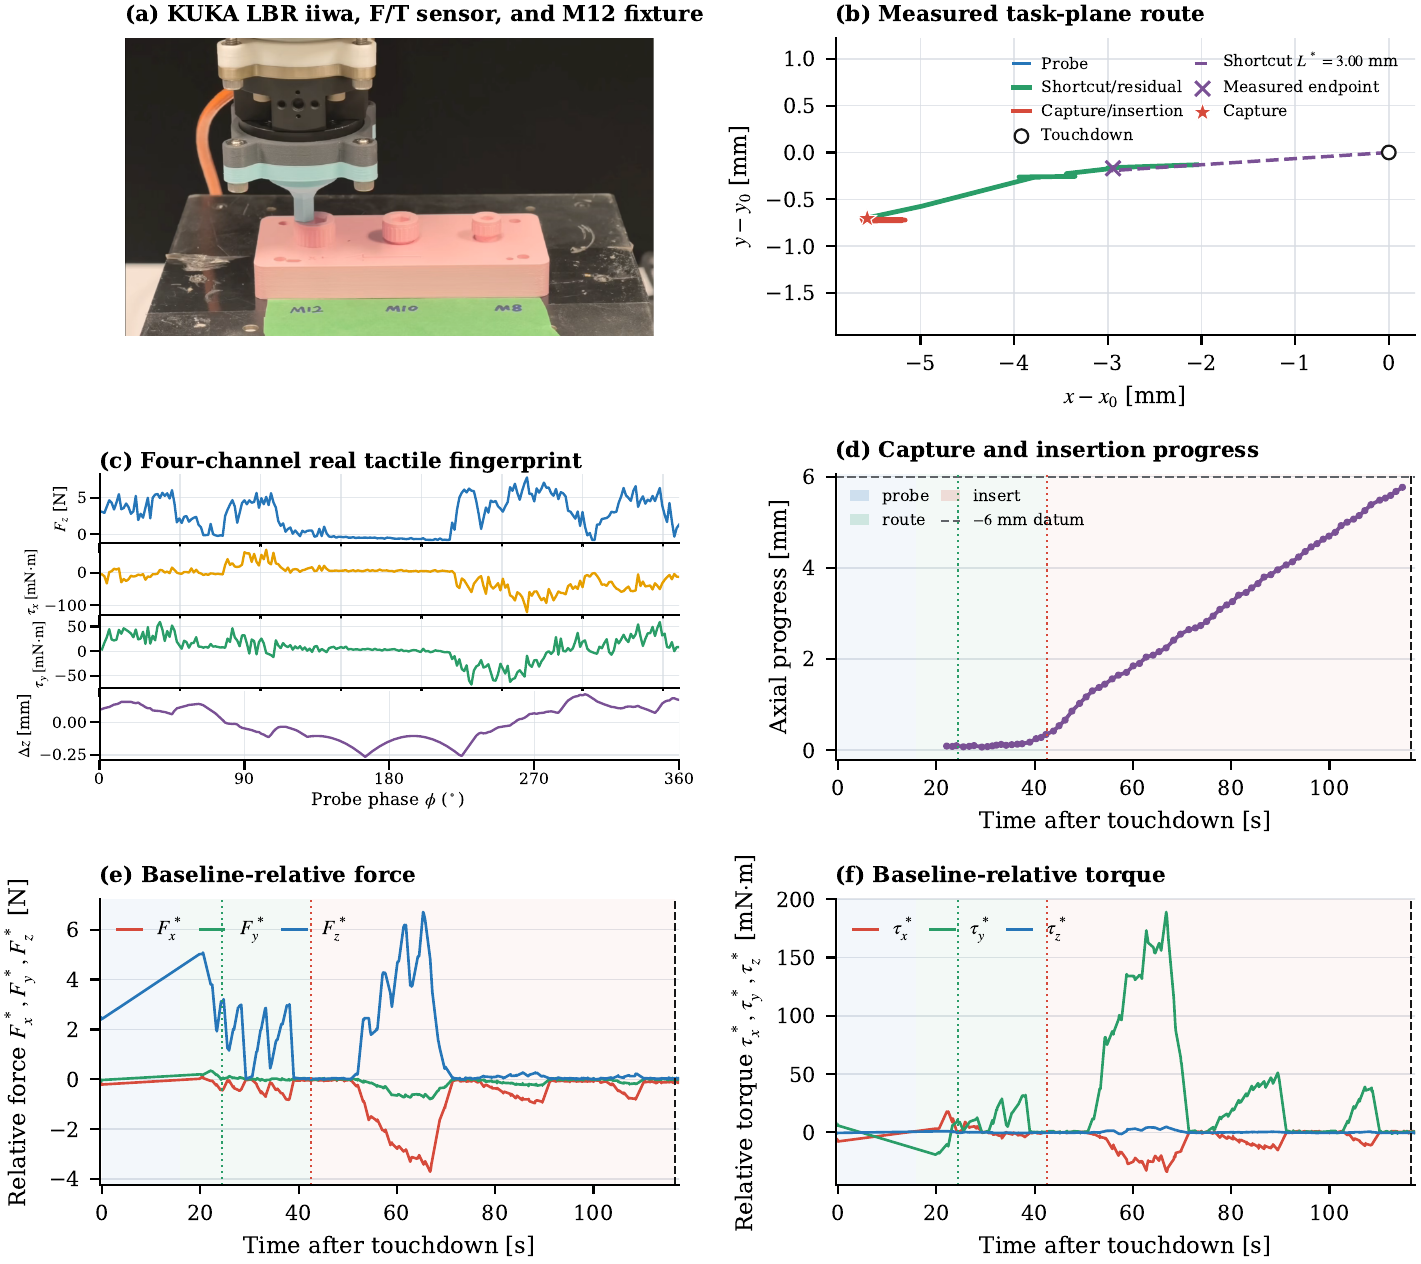
\includegraphics[width=0.97\textwidth]{figures/hardware_m12_named_feasibility.png}
  \caption{Same-run hardware evidence, one M12 \pgsg{} run.  (a) KUKA LBR
  iiwa, Bota F/T sensor, hex driver, multisize fixture.  (b) Measured
  task-plane route, with the commanded shortcut, the measured endpoint, and
  the confirmed capture.  (c) The 240-sample four-channel signal; tip
  height is centered on its scan mean for display.  (d) Axial progress from
  the touchdown height, with the $-6$~mm reference line.  (e),(f)
  Baseline-relative force and torque at the Bota origin.  Blue, green, and
  red shading mark probe, route, and insertion.  Dotted lines mark the
  negative evidence and the confirmed capture.  The black dashed line marks
  the terminal event.  Every curve here is a raw, unsmoothed timestamped
  record.  The wrench has not been moved to the tool tip or corrected
  against a certified gravity model.}
  \label{fig:hardware}
\end{figure*}

Figure~\ref{fig:hardware_pair} lines up two runs from the same starting
point.  These are only mechanism checks.  Two runs cannot give a success
rate.  \pgsg{} rejects the endpoint of its bounded shortcut and clears the
rest of the route after one conical touch.  Direct-4C misses on its first
ray, probes again, and then captures.  Both eventually reach the terminal
state, under an extended time limit, so their paths, loads, and event logs
can all be checked on the real robot.

\begin{figure*}[t]
  \centering
  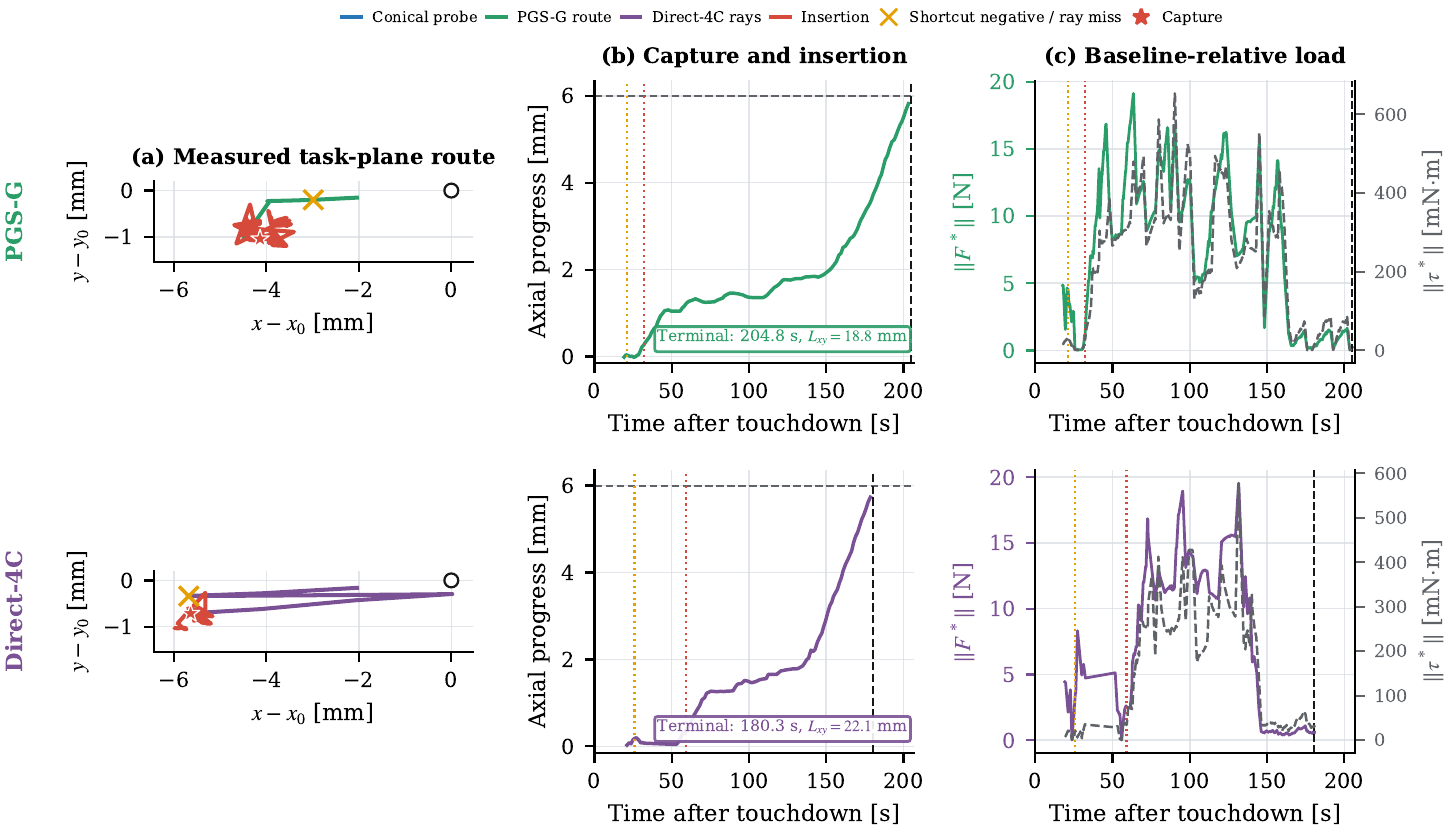
\includegraphics[width=0.97\textwidth]{figures/hardware_m12_same_start_mechanism_pair.png}
  \caption{Hardware mechanism comparison, two M12 runs from the same
  starting point.  Rows: \pgsg{}, Direct-4C.  (a) Measured task-plane route
  from each touchdown.  Circles, crosses, and stars mark touchdown,
  negative evidence, and confirmed capture.  (b) Axial progress, with the
  6~mm task line.  (c) Norms of baseline-relative force and torque at the
  Bota origin.  Orange dotted, red dotted, and black dashed lines mark
  negative evidence, capture, and terminal events.  Curves are raw,
  unsmoothed records.  This pair is meant to show mechanism.  It was not
  run as a randomized comparison.}
  \label{fig:hardware_pair}
\end{figure*}

Figure~\ref{fig:hardware_matrix} lines up the full chain, from posterior to
contact, for one fixed-seed four-policy M12 run.  Every column uses the
same registered offset and the same plotting scale.  All three tactile
methods pick the same main direction here, but they split up the rest of
the route differently.  \pgsg{} uses its negative evidence to replan a
tight grid route.  \pgso{} covers the remaining region with a local spiral.
Direct-4C commits to one bounded ray.  Outward ignores the posterior and
simply expands a global spiral.  The times and paths shown belong only to
these chosen runs.  They are not an estimate of policy-level success or
speed.

\begin{figure*}[t]
  \centering
  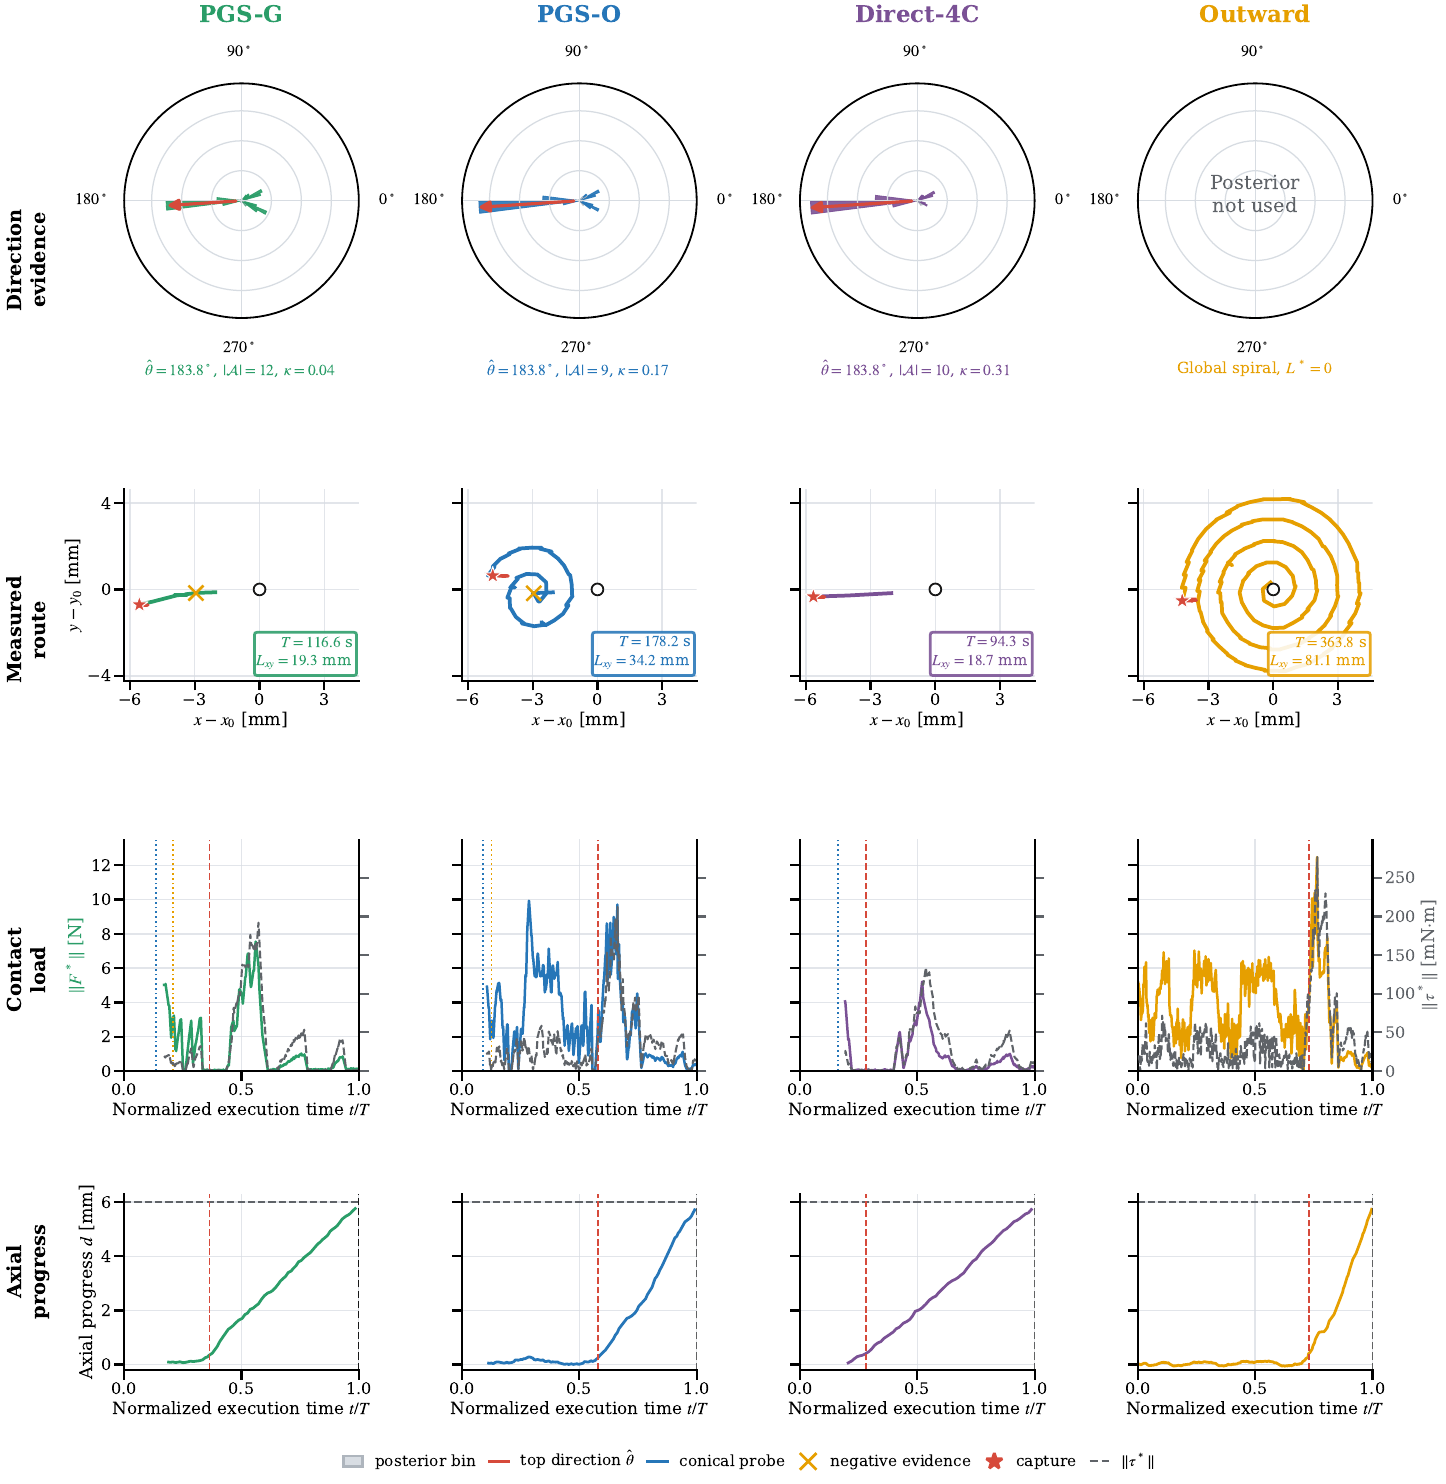
\includegraphics[width=0.98\textwidth]{figures/hardware_m12_four_policy_evidence_matrix.png}
  \caption{Perception--action--contact matrix, one fixed-seed M12 hardware
  task.  Columns: \pgsg{}, \pgso{}, Direct-4C, Outward.  Top row: the
  measured 48-bin direction posterior.  Colored bins mark the prediction
  set.  The red arrow marks the top direction.  Outward has no tactile
  posterior at all.  Second row: the measured task-plane route on shared
  axes.  The circle, orange cross, and red star mark touchdown, valid
  negative evidence, and confirmed capture.  Badges give terminal time and
  travel for that run.  Third row: force (solid, left scale) and torque
  (gray dashed, right scale), both baseline-relative, over normalized time.
  Blue dotted, orange dotted, and red dashed lines mark probe end, negative
  evidence, and capture.  Bottom row: axial progress from touchdown.  The
  gray line is the 6~mm task datum.  The black line is the terminal event.
  Every trace here is a raw, unsmoothed hardware record.  This one campaign
  was picked to show mechanism and how effort gets spent, not to serve as a
  randomized comparison.}
  \label{fig:hardware_matrix}
\end{figure*}

Table~\ref{tab:hardware_evidence} lists the hardware records used in this
paper.  The scan campaign checks acquisition across all three socket sizes.
The M12 method runs and the two M10 pilots exercise the closed loop.  These
runs came from named or fixed starts, so the table reports what was seen,
not a success rate.

\begin{table*}[t]
\caption{Hardware evidence used in the paper.  Named and fixed-start
executions serve as mechanism checks.  We do not read them as population
success rates.}
\label{tab:hardware_evidence}
\centering
\scriptsize
\setlength{\tabcolsep}{5.5pt}
\begin{tabular}{lllll}
\toprule
Size & Hardware record & Method(s) & Runs & Recorded outcome\\
\midrule
M8/M10/M12 & registered conical scans & conical acquisition & 26/size & 78/78 valid traces\\
M12 & fixed-seed method runs & \pgso{}, \pgsg{}, Outward, Direct-4C & 1/method & three terminal; Outward terminal after extension\\
M10 & fixed-start pilots & \pgsg{} & 2 & both reached terminal depth\\
\bottomrule
\end{tabular}
\end{table*}

\clearpage
\twocolumn
%%%%%%%%%%%%%%%%%%%%%%%%%%%%%%%%%%%%%%%%%%%%%%%%%%%%%%%%%%%%%%%%%%%%%%%%%%%%%%%%
\section{Discussion}

The tactile scan turns out to play a narrow role.  It changes where the
search budget gets spent.  It does not point straight at the socket center.
That is why \pgso{} routes stay short next to global outward search.  It is
also why the entropy grid barely helps here, since the residual regions
tested are small to begin with.  Recovery solves a different problem: it
puts the robot back into a searchable contact state once an insertion try
is rejected.

The gap between simulation and reality shows up mainly in the observation
model.  A model trained on the real tool sees friction, compliance, sensor
chain, and registration errors that contact rendering leaves out or
simplifies.  It does not fix session drift, wear, temperature effects, or
shifts across socket size.  That is why the learned output stays a route
proposal.  Capture is still decided from the measured contact, not from the
model.

A few limits are worth stating.  Proposition~1 covers the retained mass of
the empirical posterior under exact endpoint execution.  It gives no
guarantee once the distribution shifts.  Boundary truncation, tracking
error, or a budget that runs out can also stop a finite spiral or grid from
covering its full set.  The hardware records come from one fixture and a
set of chosen starts, so we do not infer a random-start success rate from
them.  Bota readings are relative to a same-run baseline at the sensor
origin, with no certified gravity compensation and no shift of moment to
the tool tip.  Last, the terminal dwell only confirms geometric engagement.
It says nothing about first-turn coupling, slip, thread release, or
extraction.

%%%%%%%%%%%%%%%%%%%%%%%%%%%%%%%%%%%%%%%%%%%%%%%%%%%%%%%%%%%%%%%%%%%%%%%%%%%%%%%%
\section{Conclusion}

This work treats tactile direction as partial evidence about the socket
pose.  It is not a full estimate of that pose.  A conical probe updates the
planar center belief.  The confident part of that belief becomes a capped
shortcut.  What is left goes to a finite local search.  Capture, recovery,
and the final check all run through the same compliant loop, on every
route.  On the paired M8 tasks, this setup keeps the same engagement rate
while cutting the route short, compared with an outward spiral.  The
recovery study and the M10/M12 hardware records show that this same split,
learned guidance on one side and physical checking on the other, carries
over to the real robot.  The claim made here stops at geometric
engagement.  Turning the screw, releasing the thread, and extracting it
each need their own contact rules, still to come.

\bibliographystyle{IEEEtran}
\bibliography{references}

\end{document}
